\chapter{Introdução à análise ascendente}

\section{Introdução}

Até agora, estudamos técnicas \textbf{top-down} para a análise
sintática. Um analisador sintático top-down é limitado nas gramáticas
que pode processar, pois precisa ser capaz de decidir qual regra deve
ser usada com base em relativamente pouca informação. Por exemplo,
ele precisa ser capaz de escolher a produção correta a partir do
símbolo inicial com base no primeiro token da entrada.

Essa limitação motiva a análise sintática \textbf{bottom-up}, na qual
o analisador sintático pode escolher produções após analisar um
prefixo maior da entrada. Por exemplo, os analisadores sintáticos de
bottom-up podem lidar com produções recursivas à esquerda, enquanto
os analisadores sintáticos top-down não. De fato, os analisadores
sintáticos bottom-up funcionam melhor quando as produções são
recursivas à esquerda, embora também possam lidar com produções
recursivas à direita.

Neste capítulo, vamos apresentar dois algoritmos bottom-up: o
algoritmo CYK e os algoritmos LR(0) e SLR.

\section{Forma Normal de Chomsky}

Uma gramática livre de contexto está na \textbf{Forma Normal de Chomsky} (FNC) quando toda produção tem uma das duas formas:
\[
  A \to BC \qquad \text{ou} \qquad A \to a
\]
onde $A$, $B$ e $C$ são não-terminais e $a$ é um terminal. Adicionalmente, o símbolo inicial $S$ pode ter a produção $S \to \lambda$ somente se $\lambda$ pertencer à linguagem.

A FNC simplifica muitos algoritmos sobre gramáticas livres de contexto. Em particular, o algoritmo CYK requer que a gramática de entrada esteja em FNC: como toda produção binária produz exatamente dois não-terminais, a árvore de derivação de qualquer cadeia de comprimento $n$ tem exatamente $2n - 1$ nós internos, tornando o espaço de busca finito e bem estruturado.

\subsection{Conversão para a FNC}

Toda GLC pode ser convertida para uma gramática equivalente em FNC. O processo aplica quatro transformações em sequência:

\begin{enumerate}
  \item \textbf{Novo símbolo inicial.} Acrescente $S_0 \to S$ e torne $S_0$ o novo símbolo inicial. Isso evita que $S$ apareça no lado direito de alguma produção.

  \item \textbf{Eliminação de produções vazias.} Para cada não-terminal nulável $A$ (tal que $A \Rightarrow^* \lambda$), em toda produção que contenha $A$ no lado direito, acrescente uma cópia da produção sem essa ocorrência de $A$. Depois remova $A \to \lambda$ (exceto $S_0 \to \lambda$ se $\lambda \in L(G)$).

  \item \textbf{Eliminação de produções unitárias.} Para cada produção $A \to B$ onde $B$ é um único não-terminal, adicione $A \to \gamma$ para cada produção $B \to \gamma$ e remova $A \to B$.

  \item \textbf{Binarização e terminalização.} Para produções longas $A \to X_1 X_2 \cdots X_k$ com $k \geq 3$, introduza não-terminais auxiliares: $A \to X_1 A_1$, $A_1 \to X_2 A_2$, \ldots, $A_{k-2} \to X_{k-1} X_k$. Para produções binárias $A \to X_1 X_2$ em que algum $X_i$ é um terminal $a$, introduza $N_a \to a$ e substitua $a$ por $N_a$.
\end{enumerate}

\subsection{Exemplo de conversão}

Considere a gramática para $\{a^n b^n \mid n \geq 1\}$:
\[
  S \to a\,S\,b \mid a\,b
\]

\textbf{Passo 1 — novo símbolo inicial:}
\[
  S_0 \to S, \quad S \to a\,S\,b \mid a\,b
\]

\textbf{Passo 4 — binarização e terminalização} ($S \to a\,S\,b$ tem comprimento 3 com terminais mistos):
\[
  \begin{array}{lcl}
    S_0 & \to & S \\
    S   & \to & N_a\,A_1 \mid N_a\,N_b \\
    A_1 & \to & S\,N_b \\
    N_a & \to & a \\
    N_b & \to & b
  \end{array}
\]

\textbf{Passo 3 — eliminar unitária} ($S_0 \to S$): copiar as produções de $S$ para $S_0$:
\[
  \begin{array}{lcl}
    S_0 & \to & N_a\,A_1 \mid N_a\,N_b \\
    S   & \to & N_a\,A_1 \mid N_a\,N_b \\
    A_1 & \to & S\,N_b \\
    N_a & \to & a \\
    N_b & \to & b
  \end{array}
\]

Esta gramática está em FNC e gera a mesma linguagem $\{a^n b^n \mid n \geq 1\}$.

\section{Algoritmo CYK}

O algoritmo de Cocke-Younger-Kasami (CYK) é um reconhecedor para gramáticas em FNC. Dado uma gramática $G$ em FNC e uma cadeia $w = a_1 a_2 \cdots a_n$, o CYK determina se $w \in L(G)$ em tempo $O(n^3 |G|)$, onde $|G|$ é o número de produções de $G$.

\subsection{Estrutura da tabela}

O algoritmo preenche uma tabela triangular $T$ onde a entrada $T[i][j]$ (com $1 \leq i \leq j \leq n$) contém o conjunto de não-terminais que derivam a subcadeia $a_i \cdots a_j$:
\[
  T[i][j] = \{ A \in V \mid A \Rightarrow^* a_i \cdots a_j \}
\]

A cadeia $w$ pertence a $L(G)$ se e somente se $S \in T[1][n]$.

\subsection{O algoritmo}

O preenchimento da tabela segue o princípio de \textbf{programação dinâmica}: subcadeias de comprimento menor são resolvidas primeiro e seus resultados são reutilizados para resolver subcadeias maiores.

\begin{algorithm}[H]
\caption{Algoritmo CYK}
\begin{algorithmic}[1]
\Require Gramática $G$ em FNC com símbolo inicial $S$; cadeia $w = a_1 \cdots a_n$
\Ensure \textbf{verdadeiro} se $w \in L(G)$, \textbf{falso} caso contrário
\For{$i \leftarrow 1$ \textbf{to} $n$}
  \State $T[i][i] \leftarrow \{A \mid A \to a_i \in G\}$
\EndFor
\For{$\ell \leftarrow 2$ \textbf{to} $n$}
  \For{$i \leftarrow 1$ \textbf{to} $n - \ell + 1$}
    \State $j \leftarrow i + \ell - 1$
    \State $T[i][j] \leftarrow \emptyset$
    \For{$k \leftarrow i$ \textbf{to} $j - 1$}
      \For{cada produção $A \to BC \in G$}
        \If{$B \in T[i][k]$ \textbf{e} $C \in T[k+1][j]$}
          \State $T[i][j] \leftarrow T[i][j] \cup \{A\}$
        \EndIf
      \EndFor
    \EndFor
  \EndFor
\EndFor
\Return $S \in T[1][n]$
\end{algorithmic}
\end{algorithm}

\subsection{Conexão com programação dinâmica}

O CYK é um exemplo clássico de programação dinâmica. Identificamos três componentes centrais:

\begin{itemize}
  \item \textbf{Subproblema:} calcular $T[i][j]$, o conjunto de não-terminais que derivam $a_i \cdots a_j$.
  \item \textbf{Subestrutura ótima:} se $A \Rightarrow^* a_i \cdots a_j$ pela produção $A \to BC$, então existe $k$ tal que $B \Rightarrow^* a_i \cdots a_k$ e $C \Rightarrow^* a_{k+1} \cdots a_j$. Portanto, $A \in T[i][j]$ depende apenas de $T[i][k]$ e $T[k+1][j]$, que são subproblemas estritamente menores.
  \item \textbf{Sobreposição de subproblemas:} o valor $T[i][j]$ é consultado em múltiplos subproblemas maiores. Sem memoização, o mesmo subproblema seria recomputado exponencialmente.
\end{itemize}

A tabela tem $O(n^2)$ entradas; cada entrada é calculada examinando $O(n)$ pontos de divisão $k$ e $O(|G|)$ produções binárias, resultando em complexidade total $O(n^3 |G|)$.

\subsection{Exemplo de execução}

Usamos a gramática em FNC do exemplo anterior (sem $S_0$) e analisamos $w = \texttt{aabb}$ ($n = 4$, posições $1$ a $4$):

\[
  \begin{array}{lcl}
    S   & \to & N_a\,A_1 \mid N_a\,N_b \\
    A_1 & \to & S\,N_b \\
    N_a & \to & a \\
    N_b & \to & b
  \end{array}
\]

\textbf{Passo base} (subcadeias de comprimento 1):

\begin{table}[H]
\centering
\begin{tabular}{@{}cccc@{}}
  \toprule
  $i$ & $j$ & $a_i$ & $T[i][j]$ \\
  \midrule
  1 & 1 & a & $\{N_a\}$ \\
  2 & 2 & a & $\{N_a\}$ \\
  3 & 3 & b & $\{N_b\}$ \\
  4 & 4 & b & $\{N_b\}$ \\
  \bottomrule
\end{tabular}
\end{table}

\textbf{Comprimento 2:}

\begin{table}[H]
\centering
\begin{tabular}{@{}cccl@{}}
  \toprule
  $i$ & $j$ & Subcadeia & $T[i][j]$ \\
  \midrule
  1 & 2 & \texttt{aa} & $k{=}1$: $\{N_a\}$ e $\{N_a\}$ — nenhuma produção $X \to N_a\,N_a$ — $\emptyset$ \\
  2 & 3 & \texttt{ab} & $k{=}2$: $\{N_a\}$ e $\{N_b\}$ — $S \to N_a\,N_b$ — $\{S\}$ \\
  3 & 4 & \texttt{bb} & $k{=}3$: $\{N_b\}$ e $\{N_b\}$ — nenhuma produção $X \to N_b\,N_b$ — $\emptyset$ \\
  \bottomrule
\end{tabular}
\end{table}

\textbf{Comprimento 3:}

\begin{table}[H]
\centering
\begin{tabular}{@{}cccl@{}}
  \toprule
  $i$ & $j$ & Subcadeia & $T[i][j]$ \\
  \midrule
  1 & 3 & \texttt{aab} & $k{=}1$: $\{N_a\}$ e $\emptyset$ — vazio; $k{=}2$: $\emptyset$ e $\{N_b\}$ — vazio — $\emptyset$ \\
  2 & 4 & \texttt{abb} & $k{=}2$: $\{N_a\}$ e $\emptyset$ — vazio; $k{=}3$: $\{S\}$ e $\{N_b\}$ — $A_1 \to S\,N_b$ — $\{A_1\}$ \\
  \bottomrule
\end{tabular}
\end{table}

\textbf{Comprimento 4} (cadeia completa):

\begin{table}[H]
\centering
\begin{tabular}{@{}cccl@{}}
  \toprule
  $i$ & $j$ & Subcadeia & $T[i][j]$ \\
  \midrule
  1 & 4 & \texttt{aabb} & $k{=}1$: $\{N_a\}$ e $\{A_1\}$ — $S \to N_a\,A_1$ — $\{S\}$ \\
  \bottomrule
\end{tabular}
\end{table}

Como $S \in T[1][4]$, a cadeia \texttt{aabb} é aceita. A figura abaixo mostra a árvore de derivação correspondente:

\[
  S \;\Rightarrow\; N_a\,A_1 \;\Rightarrow\; a\,A_1 \;\Rightarrow\; a\,S\,N_b \;\Rightarrow\; a\,N_a\,N_b\,N_b \;\Rightarrow\; a\,a\,b\,b
\]

\subsection{Complexidade}

\begin{itemize}
  \item \textbf{Tempo:} $O(n^3 |G|)$ — $O(n^2)$ pares $(i,j)$, $O(n)$ divisões $k$ por par, $O(|G|)$ verificações de produções.
  \item \textbf{Espaço:} $O(n^2 |G|)$ para armazenar a tabela.
  \item O CYK demonstra que o reconhecimento de GLC é sempre polinomial, contrastando com buscas recursivas ingênuas de complexidade exponencial.
\end{itemize}

\section{Analisadores LR(0) e SLR}

A análise LR, incluindo a análise LALR, é um método popular de
análise sintática. Esses algoritmos são a tecnologia subjacente em
diversos geradores de analisadores sintáticos, como o Happy. Podemos
pensar nos analisadores LR como aqueles que pré-computam toda a
estrutura de predição, codificando-a em um autômato finito determinístico.
A análise LR consiste em duas ações: shift e reduce, portanto, os
analisadores LR são chamados de analisadores de shift-reduce.

Em vez de manter o controle de todas as possíveis análises sintáticas
à direita simultaneamente, um analisador sintático de shift-reduce
mantém apenas a análise que corresponde a uma única derivação mais à
direita. Isso torna o estado do analisador muito mais simples: em
qualquer ponto da análise, o estado consiste em uma pilha de símbolos
e o estado atual da derivação é a concatenação da pilha com a entrada
não consumida. Por exemplo, podemos escrever a análise sintática da
expressão \verb|(1)+2| como uma série de operações de shift e reduce
que constroem uma derivação mais à direita inversa:

\begin{table}[H]
\begin{tabular}{@{}lll@{}}
  \toprule
  Pilha de Derivação & Ações & Entrada não consumida \\
  \midrule
  (1) + 2 & (1) + 2 & \\
  (1) + 2 & shift & (1) + 2 \\
  (1) + 2 & shift & (1) + 2 \\
  (E) + 2 & reduce E $\to$ n & (E) + 2 \\
  (S) + 2 & reduce S $\to$ E & (S) + 2 \\
  (S) + 2 & shift & (S) + 2 \\
  E + 2 & reduce E $\to$ (S) & E + 2 \\
  S + 2 & reduce S $\to$ E & S + 2 \\
  S + 2 & shift & S + 2 \\
  S + 2 & shift & S + 2 \\
  S + E & reduce E $\to$ n & S + E \\
  S & reduce S $\to$ S+E & S \\
  \bottomrule
\end{tabular}
\centering
\end{table}

Para determinar qual ação deve ser tomada em cada etapa, o analisador
sintático precisa saber quais são as possíveis produções futuras a
serem reduzidas. As possíveis produções futuras são um conjunto de
itens, fechado sob predição; esse conjunto de itens nos diz qual ação
faz sentido em um determinado ponto da análise sintática. Para mapear
uma pilha em um conjunto de itens, esses conjuntos de itens podem ser
interpretados como um autômato finito determinístico que lê a pilha e
cujos estados são exatamente os conjuntos de itens. Esses estados têm a propriedade de que,
ignorando a predição, apenas uma ação significativa pode ser tomada
em cada estado: shift ou reduce.

O estado inicial do autômato LR(0) contém os itens do símbolo de
partida aumentado, acrescido do símbolo de fim de entrada, e é
fechado sob predição.

\[
\begin{array}{l}
  S' \to . S \$\\
  S \to . S + E\\
  S \to . E\\
  E \to . n\\
  E \to . ( S )\\
\end{array}
\]

O autômato é construído repetindo-se o seguinte procedimento até que
nenhuma alteração adicional seja possível. Escolha um estado e um
símbolo que esteja à direita do ponto em uma ou mais produções.
Desloque esse símbolo para a direita nesses itens e feche o conjunto
de itens sob previsão. O conjunto de itens resultante pode ser um
estado existente do autômato ou um novo. Em ambos os casos, adicione
uma transição no símbolo escolhido do estado antigo para o estado
correspondente a este conjunto de itens.

\begin{figure}[H]
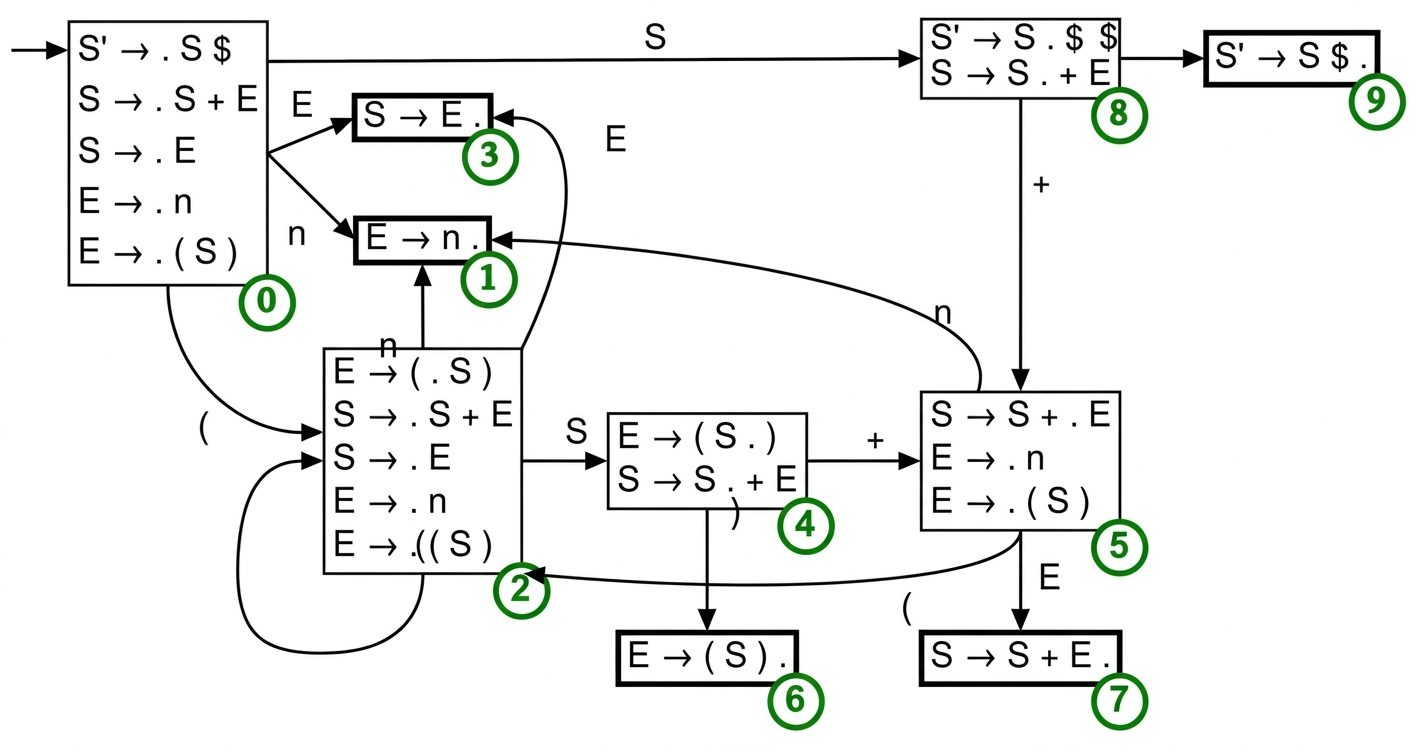
\includegraphics[scale=0.2]{./chapters/lr0.png}
\centering
\end{figure}

Por exemplo, ao realizar uma transição no token ( do estado inicial,
deslocamos apenas o último item para a direita, obtendo um estado
contendo a produção \(E \to ( . S )\), sobre o qual então realizamos
um fechamento de predição que adiciona itens para \(S\) e, em
seguida, para \(E\). Ao realizar uma transição a partir do mesmo
estado no não terminal S, deslocamos os dois primeiros itens para a
direita, obtendo os itens $S' \to S . \$$ e \(S \to S.+E\). O
fechamento de predição não adiciona nenhum item a este estado. A
figura a seguir mostra os passos que você pode seguir para completar
o autômato (pressione o botão para avançar a animação). Na figura, os
estados estão numerados em verde e os estados nos quais uma ação de
redução deve ser realizada têm uma borda mais espessa.

Podemos resumir este autômato em duas tabelas que podem ser usadas
para controlar um analisador sintático. A primeira é a tabela action,
que informa ao analisador o que fazer em cada estado, dado o símbolo
de previsão: shift e ir para um novo estado, ou reduce por alguma
produção. A segunda tabela é a tabela goto, que informa ao analisador
para qual estado ir quando ele reduz uma produção. Abaixo estão essas
duas tabelas do autômato que acabamos de construir, lado a lado.
Entradas vazias nas tabelas correspondem a erros de sintaxe. Entradas
numéricas na tabela action correspondem a ações de shift; uma
produção na tabela action indica uma ação de reduce.

\begin{table}[H]
  \begin{tabular}{@{}llllllll@{}}
    \toprule
    & n & + & ( & ) & \$ & S & E \\
    \midrule
    0 & 1 & & 2 & & & 8 & 3 \\
    1 & E $\to$ n & E $\to$ n & E $\to$ n & E $\to$ n & E $\to$ n & & \\
    2 & 1 & & 2 & & & 4 & 3 \\
    3 & S $\to$ E & S $\to$ E & S $\to$ E & S $\to$ E & S $\to$ E & & \\
    4 & & 5 & & 6 & & & \\
    5 & 1 & & 2 & & & & 7 \\
    6 & E $\to$ (S) & E $\to$ (S) & E $\to$ (S) & E $\to$ (S) & E
    $\to$ (S) & & \\
    7 & S $\to$ S+E & S $\to$ S+E & S $\to$ S+E & S $\to$ S+E & S
    $\to$ S+E & & \\
    8 & & 5 & & & 9 & & \\
    9 & \(S'\to S\). & \(S' \to S\). & \(S'\to S\). & \(S' \to S\). & \(S'\to
    S\$\). & & \\
    \bottomrule
  \end{tabular}
  \centering
\end{table}

Durante sua execução, um analisador sintático shift-reduce utiliza
uma tabela (como a apresentada) e uma pilha de estados. O algoritmo
inicia com a pilha contendo o estado inicial e a entrada a ser
processada. À medida que lê cada token de entrada, ele consulta na
tabela action qual é a ação atual para o estado no topo da pilha,
dado o próximo token. Se a ação for um shift, ele adiciona o estado
especificado à pilha. Se a ação for um reduce, ele remove da pilha o
número de itens na produção correspondente e usa a tabela goto do
estado agora no topo da pilha para determinar o próximo estado a ser
adicionado à pilha.

Vamos testar este analisador sintático no exemplo anterior,
\verb|(1)+2|. A pilha contém apenas o estado 0.
Para tornar mais claro, os estados na pilha são mostrados em
\textbf{negrito} e são precedidos pelo símbolo que foi seguido para
chegar a esse estado. Esses símbolos correspondem à parte da
derivação que foi construída até agora pelo analisador sintático.
\begin{table}[H]
  \begin{tabular}{@{}lll@{}}
    \toprule
    Pilha & Entrada & Ação \\
    \midrule
    \textbf{0} & (1)+2 & shift \textbf{2} \\
    \textbf{0}(\textbf{2} & 1)+2 & shift \textbf{1} \\
    \textbf{0}(\textbf{21} & )+2 & reduce E $\to$ n \\
    \textbf{0}(\textbf{2}E\textbf{3} & )+2 & reduce S $\to$ E \\
    \textbf{0}(\textbf{2}S\textbf{4} & )+2 & shift \textbf{6} \\
    \textbf{0}(\textbf{2}S\textbf{4})\textbf{6} & +2 & reduce E $\to$ (S) \\
    \textbf{0}E\textbf{3} & +2 & reduce S $\to$ E \\
    \textbf{0}S\textbf{8} & +2 & shift \textbf{5} \\
    \textbf{0}S\textbf{8}+\textbf{5} & 2 & shift \textbf{1} \\
    \textbf{0}S\textbf{8}+\textbf{51} & \$ & reduce E $\to$ n \\
    \textbf{0}S\textbf{8}+\textbf{5}E\textbf{7} & \$ & reduce S $\to$ S+E \\
    \textbf{0}S\textbf{8} & \$ & shift \textbf{9} \\
    \textbf{0}S\textbf{8}\$\textbf{9} & & reduce S' $\to$ S \\
    \bottomrule
  \end{tabular}
  \centering
\end{table}

Note que a construção LR que vimos até agora não faz nada além de
reduzir a uma única produção fixa, independentemente do próximo token
na entrada. Como resultado, os estados que contêm reduções (estados
1, 3, 6, 7, 9 no exemplo) ignoram o token de lookahead. A esse
algoritmo damos o nome de analisador LR(0). Preenchendo as tabelas de
action e goto de uma maneira menos restritiva, poderíamos obter um
analisador LR(1), que é mais expressivo. No entanto, precisaremos
modificar a construção da tabela LR(0) que acabamos de ver para obter
essa expressividade.

Uma extensão simples, mas surpreendentemente eficaz, para LR(0) é
adicionar uma ação de redução à tabela de ações apenas no caso em que
o token de lookahead esteja no conjunto FOLLOW do não terminal que
está sendo reduzido, já que, caso contrário, a produção claramente
não leva a uma análise válida. Quando esse refinamento na construção
LR(0) produz um analisador sintático shift-reduce válido, dizemos que
a gramática é SLR (Simple LR).

\section{Implementação}

Nesta seção comentamos os principais detalhes das implementações
Haskell dos algoritmos apresentados neste capítulo.

\subsection{Algoritmo CYK}

A implementação está no módulo \verb|Parsing.CYK.CYKParser|.
Os tipos principais refletem diretamente a tabela triangular do algoritmo.

\subsubsection{Representação da tabela}

A tabela CYK mapeia pares $(i, j)$ ao conjunto de não-terminais que derivam $a_i \cdots a_j$:

\begin{minted}{haskell}
type CYKTable = Map (Int, Int) (Set String)
\end{minted}

\subsubsection{Construção da tabela}

A função \haskell{buildTable} implementa o algoritmo em dois estágios. Primeiro, preenche as células diagonais (comprimento 1):

\begin{minted}{haskell}
base = Map.fromList
    [ ((i, i), Set.fromList
          [ lhs
          | (lhs, prods) <- Map.toList g
          , [Terminal tok] `elem` prods
          ])
    | (i, tok) <- indexed
    ]
\end{minted}

Em seguida, percorre os pares $(i, j)$ em ordem crescente de comprimento $j - i + 1$ e preenche cada célula consultando as células já calculadas:

\begin{minted}{haskell}
spans = [ (i, i + l - 1)
        | l <- [2..n]
        , i <- [1..n - l + 1]
        ]

fillSpan tbl (i, j) =
    let new = Set.fromList
                [ lhs
                | k <- [i..j-1]
                , let bs = look (i, k)   tbl
                , let cs = look (k+1, j) tbl
                , not (Set.null bs || Set.null cs)
                , (lhs, b, c) <- binaryProds
                , Set.member b bs
                , Set.member c cs
                ]
    in Map.insertWith Set.union (i, j) new tbl
\end{minted}

A ordem de enumeração em \haskell{spans} garante que, ao calcular $T[i][j]$, todos os valores $T[i][k]$ e $T[k+1][j]$ (com $k < j - i$) já estejam disponíveis na tabela — essa é a propriedade central da programação dinâmica.

\subsubsection{Reconhecimento}

\begin{minted}{haskell}
cykParse :: Grammar -> String -> [String] -> CYKResult
cykParse g start tokens
    | null tokens              = if acceptsEmpty then CYKAccept
                                                 else CYKReject
    | Set.member start topCell = CYKAccept
    | otherwise                = CYKReject
  where
    n        = length tokens
    tbl      = buildTable g tokens
    topCell  = fromMaybe Set.empty (Map.lookup (1, n) tbl)
    acceptsEmpty = any isEpsilon (fromMaybe [] (Map.lookup start g))
    isEpsilon p  = null p || p == [Terminal "\955"]
\end{minted}

A condição de aceitação verifica se \haskell{start} pertence à célula $(1, n)$, correspondendo exatamente a $S \in T[1][n]$ do algoritmo.

\subsection{LR(0) e SLR}

A implementação está distribuída em três módulos:
\begin{flushleft}
  \verb|Parsing.LR.LR0.BuildTable|,\\
  \verb|Parsing.LR.LR0.LR0Parser| e\\
  \verb|Parsing.LR.SLR.BuildTable|.
\end{flushleft}

\subsubsection{Itens e estados LR(0)}

Um item LR(0) \(A \to \alpha . \beta\) não carrega posição de origem: os estados do autômato já capturam essa informação implicitamente:

\begin{minted}{haskell}
data Item = Item
  { itemLHS :: String    -- não-terminal
  , itemBefore :: [Symbol]  -- símbolos antes do ponto
  , itemAfter :: [Symbol]  -- símbolos depois do ponto
  }

type State = Set Item
\end{minted}

Um estado LR(0) é um conjunto de itens, exatamente como os conjuntos
de itens apresentados na seção anterior. O autômato cujos estados são
esses conjuntos é o DFA que lê a pilha do analisador.

\subsubsection{Fechamento e transições}

A função \haskell{closure} implementa o fechamento de
predição descrito no capítulo: para cada item com um não-terminal
\(C\) após o ponto, adiciona todos os itens \(C \to . \gamma\):

\begin{minted}{haskell}
closure :: Grammar -> State -> State
closure g = fixedPoint step
  where
    step current = Set.union current $ Set.fromList
        [ Item b [] prod
        | item <- Set.toList current
        , NonTerminal b <- take 1 (itemAfter item)
        , prod <- fromMaybe [] (Map.lookup b g)
        ]
\end{minted}

A função \haskell{goto} computa a transição do
autômato ao consumir um símbolo: avança o ponto nos itens que têm
esse símbolo imediatamente após ele e fecha o resultado:

\begin{minted}{haskell}
goto :: Grammar -> State -> Symbol -> State
goto g items sym = closure g $ Set.fromList
    [ Item lhs (before ++ [sym]) rest
    | Item lhs before (s:rest) <- Set.toList items
    , s == sym
    ]
\end{minted}

A função \haskell{buildStates} constrói a coleção
canônica de estados LR(0) por busca em largura, partindo do estado
inicial que contém o item \(S' \to . S\) da gramática aumentada:

\begin{minted}{haskell}
buildStates :: Grammar -> [State]
buildStates g = buildFrom [initial] [initial]
  where
    initial = closure g' (Set.singleton $ initialItem g')
    buildFrom seen [] = seen
    buildFrom seen (cur : queue) =
        let newStates = [goto g' cur sym | sym <- nextSymbols cur]
            unseen    = filter (`notElem` seen) newStates
        in buildFrom (seen ++ unseen) (queue ++ unseen)
\end{minted}

\subsubsection{Tabela de parsing LR(0)}

A tabela de parsing tem duas partes: a tabela
\haskell{action}, que mapeia
\haskell{(estado, terminal)} para uma ação, e a
tabela \haskell{goto}, que mapeia
\haskell{(estado, não-terminal)} para o próximo
estado após uma redução:

\begin{minted}{haskell}
data Action = Shift Int | Reduce String [Symbol] | Accept

data ParsingTable = ParsingTable
  { actionTable :: Map (Int, String) Action
  , gotoTable :: Map (Int, String) Int
  , states :: [State]
  }
\end{minted}

O preenchimento da tabela segue as regras descritas na seção de LR(0):

\begin{itemize}
  \item
    \textbf{Shift}: para cada terminal \(t\) após o ponto em algum
    item de um estado \(i\), action[i, t] = Shift j, onde
    \(j\) é o índice do estado
    \haskell{goto(i, t)}.
  \item
    \textbf{Reduce (LR(0))}: para cada item completo \(A \to \alpha
    .\) em um estado \(i\), action[i, t] =
    Reduce($A \to \alpha$) para \textbf{todos} os terminais \(t\) da
    gramática. Esta é a característica do LR(0): ele ignora o
    lookahead nas reduções.
  \item
    \textbf{Accept}: quando o item completo é \(S' \to S .\),
    action[i, \$] = Accept.
\end{itemize}

\subsubsection{O algoritmo de parsing LR(0)}

O algoritmo de parsing mantém uma pilha de estados e processa a
entrada símbolo a símbolo. O tipo
\haskell{ParserState} encapsula o estado completo do analisador:

\begin{minted}{haskell}
data ParserState = ParserState
  { stateStack :: [Int] -- pilha de estados
  , symbolStack :: [Symbol]  -- pilha de símbolos (para diagnóstico)
  , inputBuffer :: [String]  -- entrada restante
  }
\end{minted}

A função \haskell{parseStep} executa um único passo:
consulta action[estado\_topo, token] e
aplica a ação correspondente:

\begin{itemize}
  \item
    \textbf{Shift n}: empilha o estado \haskell{n} e
    avança na entrada.
  \item
    \textbf{Reduce $A \to \alpha$}: desempilha $\alpha$
    estados e empilha o estado dado por
    goto[novo\_topo, A]. Depois chama
    \haskell{parseStep} recursivamente pois a entrada
    não é consumida em reduções.
  \item
    \textbf{Accept}: sinaliza sucesso.
\end{itemize}

\begin{minted}{haskell}
parseLR0 :: Grammar -> ParsingTable -> [String] -> ParseResult
parseLR0 g table tokens = go (ParserState [0] [] (tokens ++ ["$"]))
\end{minted}

\subsubsection{A diferença do SLR}

O módulo \verb|Parsing.LR.SLR.BuildTable|
reutiliza toda a infraestrutura de LR(0):
\haskell{buildStates},
\haskell{closure}, \haskell{goto},
\haskell{parseLR0}. A implementação do SLR modifica apenas a geração
das entradas de redução. Enquanto LR(0) adiciona Reduce para todos os
terminais, SLR restringe às entradas cujo terminal pertence a
\(\mathrm{FOLLOW}(A)\):

\begin{minted}{haskell}
-- LR(0): reduz em todos os terminais
reduceA = [ ((i, t), Reduce lhs alpha)
          | item <- Set.toList state, null (itemAfter item)
          , t <- terminals g ++ ["$"] ]

-- SLR: reduz apenas nos terminais em FOLLOW(lhs)
reduceA = [ ((i, t), Reduce lhs alpha)
          | item <- Set.toList state, null (itemAfter item)
          , t <- fromMaybe [] (Map.lookup lhs followSets) ]
\end{minted}

Esta mudança pontual é suficiente para que a gramática de expressões
\[
  \begin{array}{lcl}
    E & \to  & E + T \\
    & \mid & T \\
    T & \to  & T * F \\
    & \mid & F \\
    F & \to  & (E) \\
    & \mid & n
  \end{array}
\]
deixe de ter conflitos: no estado que contém \(E \to T.\) e \(T
\to T.*F\), LR(0) colocaria Reduce \(E \to T\) em
$*$, gerando um conflito com Shift. Com SLR,
como \(* \notin \mathrm{FOLLOW}(E) = \{+, ), \$\}\), a entrada
action[estado, *] recebe apenas Shift, não resultando em conflito.

\section{Conclusão}

Este capítulo explorou técnicas bottom-up para análise sintática, destacando como estas oferecem maior expressividade ao lidar com recursão à esquerda e prefixos mais longos da entrada. Apresentamos a Forma Normal de Chomsky como pré-requisito para o algoritmo CYK, que reconhece qualquer gramática livre de contexto em tempo $O(n^3 |G|)$ mediante programação dinâmica sobre uma tabela triangular. Em seguida, introduzimos os fundamentos da análise LR(0) e SLR, que pré-computam toda a estrutura de predição em um autômato finito determinístico, obtendo analisadores de tempo linear para a maioria das gramáticas encontradas na prática. O SLR melhora o LR(0) restringindo as ações de redução aos terminais em $\mathrm{FOLLOW}(A)$, eliminando muitos conflitos. Para superar as limitações remanescentes do SLR em gramáticas mais complexas, o próximo capítulo abordará os algoritmos LR(1) e LALR.
